\documentclass[a4paper,11pt]{article}

\usepackage[spanish]{babel}
\usepackage[utf8]{inputenc}
\usepackage{hyperref}
\usepackage{graphicx}
\usepackage{amsmath}
\graphicspath{{images/}} 

\author{Daniel Monjas Miguélez}
\title{FR: Tema 2}

\begin{document}
\begin{titlepage}
\centering
    \vfill
    {\bfseries\Large
        Fundamentos de Bases de Datos: Tema 2\\
        28 de Noviembre del 2020\\
        A year to Forget \\
        \vskip2cm
        Daniel Monjas Miguélez\\
    }    
    \vfill
    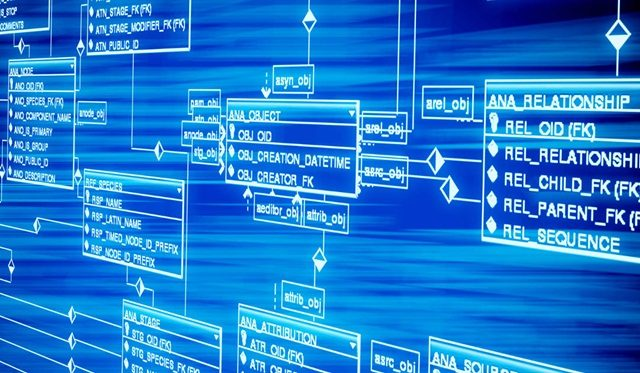
\includegraphics[width=13cm]{bases_datos.jpg}
    \vfill
    \vfill
\end{titlepage}

\newpage
\tableofcontents
\newpage

\section{Definición de modelo de datos}
\textbf{Definición formal:} mecanismo formal para representar y manipular información de manera general y sistemática. Debe constar de notación para describir datos, notación para describir operaciones y notación para describir reglas de integridad. \\

\textbf{Proceso de transformación:}

\begin{itemize}
\item Mundo real: se delimitan objetivos, se seleccionan datos, se hacen hipótesis semánticas y se organizan los datos a almacenar.

\item Esquema inicial: Se identifican los datos operativos (atributos, conexiones y restricciones).
\end{itemize}

\textbf{Historia:} El primer modelo relacional fue dieseñado por Edgar Frank Codd. Se recuperaron los modelos basados en grafos (1974). Peter Chen crea en 1975 el modelo entidad relación, y surgen otros modelos semánticos, como los modelos orientados a objetos (1983, 1986,...) y modelos lógicos (1986...). \\

\textbf{Modelado lógico:} trasladamos a un esquema lógico en función de una estructura implementable. Este modelo será implementado en un sistema comercial.

\begin{figure}
\centering
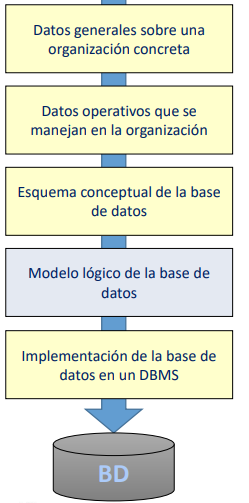
\includegraphics[scale=1,width=0.8\textwidth]{definicion_modelo_datos.png}
\caption{Pasos en la definición de una base de datos}
\end{figure}

La necesidad de modelos de datos se basa en que cada esquema se describe utilizando un lenguaje de definición de datos, este lenguaje es de muy bajo nivel y está muy ligado al SGBD y hacen falta otros mecanismos de más alto nivel que permitan describir datos de una forma no ambigua y entendible por los usuarios en cada paso del proceso de implantación. \\

El objetivo es describir modelos que representen los datos y los describan de una forma entendible y manipulable. Veamos la relación de los modelos de datos con la Arquitectura ANSI/SPARC:

\begin{itemize}
\item Nivel externo: modelo de datos externo
\item Nivel conceptual: modelo de datos conceptual
\item Nivel interno: modelo de datos interno.
\end{itemize}

Clasificaremos los modelos de datos en basados en registros, basados en objetos y físico. En cuanto a su utilización, los dos primeros se basan en los niveles externo y conceptual y el último se basa en el nivel interno. \\

\textbf{Modelos de datos basados en registros:}
\begin{itemize}
\item Modelo de datos jerárquico
\item Modelo de datos en red
\item Modelo de datos relacional (Codd, 1969)
\end{itemize}

\section{Modelo de datos relacional}
El modelo de datos relacional organiza y representa los datos en forma de tablas o relaciones. Por tanto, una base de datos relacional es una colección de tablas donde cada una de las cuales tiene un nombre único.

\begin{figure}[h]
\centering
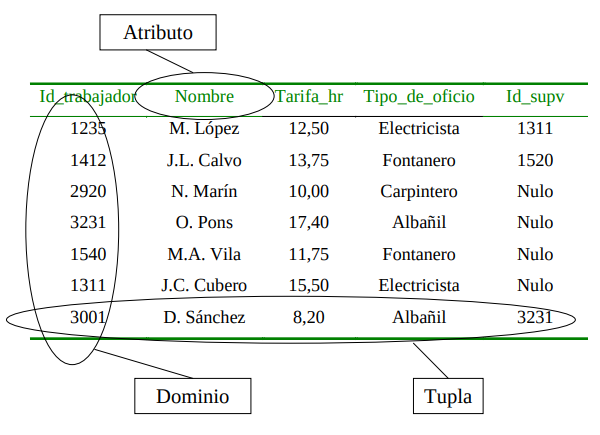
\includegraphics[scale=1,width=0.8\textwidth]{ejemplo_tabla.png}
\caption{Ejemplo tabla del modelo de datos relacional}
\end{figure}

\textbf{Conceptos:}
\begin{itemize}
\item \textbf{Esquema de una base de datos relacional:} colección de esquemas de relaciones junto con restricciones de integridad.

\item \textbf{Instancia o estado de una base de datos:} colección de instancias de relaciones que verifican las restricciones de integridad.

\item \textbf{Base de datos relacional:} instancia de una base de datos junto con su esquema.
\end{itemize}

Como ya hemos dicho el modelo de datos relacional fue introducido por Edgar Frank Codd en 1969-1970. El modelo relacional abarca tres ámbitos distintos de los datos:

\begin{itemize}
\item Las estructuras para almacenarlos: el usuario percibe la información de la base de datos estructurada en tablas.

\item La integridad: las tablas deben satisfacer ciertas condiciones que preservan la integridad y la coherencia de la información que contienen.

\item Consulta y manipulación: los operadores empleados por el modelo se aplican sobre tablas y devuelven tablas.
\end{itemize}

La tabla es la estructura lógica de un sistema relacional. A nivel físico, el sistema es libre de almacenar los datos en el formato más adecuado (archivo secuencial, archivo indexado, listas con apuntadores,...). A continuación veremos la definición formal de algunos componentes del sistema relacional:

\begin{itemize}
\item \textbf{Atributo:} cualquier elemento de información susceptible de tomar valores. Notación: $A_i, \> i=1,2,\ldots$

\item \textbf{Dominio:} rango de valores donde toma sus datos un atributo. Se considera finito. Notación: $D_i, \> i=1,2,\ldots$

\item \textbf{Relación:} dados los atributos $A_i, \> i=1,2,\ldots,n$ con dominios $D_i, \> i=1,2,\ldots,D_n$, no necesariamente distintos, definimos la relación asociada a $A_1,\ldots,A_n$, y lo notaremos por $R(A_1,\ldots,A_n)$, a cualquier subconjunto del producto cartesiano $D_1\times D_2 \times \ldots \times D_n$.

\item \textbf{Tupla:} cada una de las filas de una relación.

\item \textbf{Cardinalidad de una relación:} número de tuplas que contiene. Variable con el tiempo

\item \textbf{Esquema de una relación R:} Atributos $A_1:D_1,\ldots,A_n:D_n$

\item \textbf{Grado de una relación:} es el número de atributos de su esquema y es invariable en el tiempo.

\item \textbf{Instancia de una relación:} conjunto de tuplas $\{(x_1,x_2,\ldots,x_n)\}\subseteq D_1\times D_2 \times \ldots \times D_n$ que la componen en cada momento.
\end{itemize}

Veamos las propiedades del modelo relacional:

\begin{itemize}
\item \textbf{Condición de normalización:} todos los valores de los atributos de una relación son atomáticos, donde se dice por valor atómico un valor no estructurado. Cuando una relación cumple la primera condición de normalización se dice que está en Primera Forma Normal.
\end{itemize}

Como consecuencia no hay valores tipo conjunto, no hay valores tipo registro, ni hay valores tipo tablas. El problema es que todas las representaciones son extensivas, es decir no se puede representar directamente información del tipo 'el valor del atributo asignaturas de una lumno es: (FBD,ALG,LD)'. \\

Como consecuencias de la definición tenemos que no hay tuplas duplicadas por la definición conjuntista de relación, no hay orden en las filas ni en los atributos (al no estar ordenados ni los atributos ni las filas(conjuntos) el acceso es por Nombre de Atributo y Valor) y varias instancias representan la misma relación.

\begin{figure}[h]
\centering
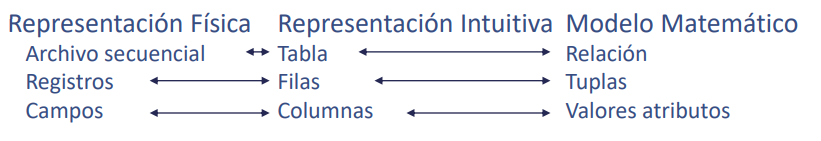
\includegraphics[scale=1,width=1\textwidth]{representacion_tabla.png}

\caption{Relacion entre la representación física, la intuitiva y el modelo matemático}
\end{figure}

\textbf{Notación a utilizar:}

\begin{itemize}
\item Relacion: $R,S,T,\ldots$
\item Atributos: $A,B,\ldots$
\item Esquema de relacion:$R[A_1,A_2,\ldots,A_n]$
\item Instancia de relación: $R:r\ldots$
\item Tuplas de una instancia:$x_1,x_2,\ldots \in r$
\item Valor de un atributo $A_i$ en una tupla $x_j:x_j[A_i] \> o \> A_{ij}$
\end{itemize}

A veces no se conoce el valor de un atributo para una determinada tupla. En esos casos a ese atributo de esa tupla se le asigna un valor nulo (un valor desconocido, un atributo no aplicable). En cualquier caso, ese valor es más de todos los dominios de la base de datos. \\

Las restricciones o reglas de integridad son condiciones para preservar la semántica de una base de datos. Estas pueden ser o bien específicas del problema ($0 \leq edad \leq 100$) o bien propias del papel de los atributos del esquema ($imparte.NRP \in profesor.NRP$ (un profesor inexistente no puede impartir una asignatura)). \\

\textbf{Superclaves y claves(candidatas y primarias):}
\begin{itemize}
\item Superclave: cualquier conjunto de atributos que identifica unívocamente a cada tupla de la relación.

\item Clave (candidata): superclave minimal, es decir, aquella con el menor número de atributos necesarios para identificar unívocamente a un tupla.
\end{itemize}

De entre las candidatas (si hubiera maś de una), hay que elegir una como principal que se denomina clave primaria. El criterio de selección puede ir en función del tamaño, significado, capacidad para recordarla,...\\

\textbf{Clave candidata y primaria (definición formal):}

\begin{itemize}
\item Sea $R[A_1,A_2,\ldots,A_n], \> CK \subseteq \{A_1,A_2,\ldots,A_n\}$ se denomina clave candidata si y sólo si:

	\begin{itemize}
		\item Unicidad: $\forall r$ instancia de R y $\forall t_1,t_2\in r \> t_1 \neq t_2 \> \Rightarrow t_1[CK]\neq t_2[CK]$
		
		\item Minimalidad: No existe CK'$\subset$CK que verifique la unicidad.
	\end{itemize}
	
, es decir, una clave candidata es un atributo o conjunto de atributos que identifica a cada tupla en la relación y que, además, no existe un subconjunto de ellos que también identifique a cada tupla de la relación.

\item Una clave primaria es la clave candidata elegida por el diseñador para desempeñar el papel de identificar. Si CK verifica la unicidad y no la minimalidad, entonces solo es superclave.
\end{itemize}

\textbf{Conceptos generales:}
Se dice condiciones de integridad a aquellas normas que mantienen la corrección semántica de una base de datos. Nos centramos en integridad genérica, la cual depende del papel que juegue un atributo en el diseño de la tabla. Son metarreglas (general las reglas de integridad aplicadas a una base de datos concreta). Existe integridad de entidad y la integridad referencial.

\begin{itemize}
\item \textbf{Integridad de entidad:} no se debe permitir que una entidad sea representada en la base de datos si no se tiene un información completa de los atributos que son clave primaria de la entidad, es decir, la clave primaria, o una parte de la misma, no puede ser un valor nulo. \\

\textbf{Clave externa (ajena):} conjunto de atributos en una relación que es una clave en otra (o incluso en la misma) relación. Podemos ver una clave externa como un conjunto de atributos de una relación cuyos valores en las tuplas deben coincidir con valores de la clave primaria de las tuplas de otra relación. \\

\textbf{Formalmente}:Clave externa $\rightarrow$ Sean $R[A_1,A_2,\ldots,A_n]$, y $PK\subseteq \{A_1,A_2,\ldots,A_n\}$ su clave primaria, sea $S[B_1,B_2,\ldots,B_n]$, y $FK\subseteq \{B_1,B_2,\ldots,B_n\}$ de amnera que card(PK)=card(FK). FK es clave externa de S con respecto a R si verifica que:
	\begin{itemize}
		\item $\forall r$ instancia de R y $\forall S$ instancia de S, $\forall x \in s \Rightarrow \exists y\in r / x[FK]=y[PK]$
		\item Es decir, el 'dominio activo' de FK debe estar incluido en el 'dominio activo' de PK para cualquier instancia de la base de datos.(Dominio activo de un atributo= valores presentes en una tabla en un momento determinado).
	\end{itemize}
	
\begin{figure}[h]
\centering
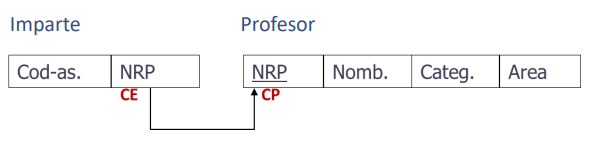
\includegraphics[scale=1,width=1\textwidth]{ejemplo_clave_externa.png}
\caption{Ejemplo clave externa}
\end{figure}

\item \textbf{Integridad referencial:} una base de datos en la que todos los valores no nulos de una clave externa referencian valores reales de la clave referenciada en la otra relación cumple la regla de integridad referencial. La integridad referencial mantiene las conexiones en las bases de datos relacionales. Puede haber más de una clave externa en una relación y puede haber una clave externa a la clave primaria de la propia relación.

\begin{figure}[h]
\centering
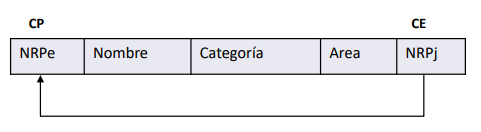
\includegraphics[scale=1,width=0.8\textwidth]{ejemplo_integridad_referencial.png}
\caption{Ejemplo de integridad referencial}
\end{figure}
\end{itemize}

El SGBD debe encargarse de mantener las siguientes restricciones:

\begin{itemize}
\item La unicidad de la clave primaria y de las claves candidatas. Frente a operaciones de inserción y actualización , el SGBD debe rechazar los valores introducidos que sean iguales a los presentes en la BD para los atributos que el diseñador ha definido como clave primaria y claves candidatas.

\item La restricción de integridad de identidad. Frente a operaciones de Inserción y Actualización, el SGBD debe rechazar las modificaciones que vulneren la unicidad en la clave primaria y/o que asignen un valor NULO a algún atributo de la clave primaria.
\end{itemize}

Veamos la integridad referencial en las siguientes operaciones:

\begin{itemize}
\item \textbf{En inserción:} rechazar la tupla insertada si el valor de la clave externa no concuerda en la relación referenciada para alguna tupla en el valor su clave primaria. Si el valor para la clave externa es NULO y el diseño no lo permite habrá de rechazar también esa inserción.

\item \textbf{En actualización:} si se actualiza la clave externa, rechazar la modificación si se produce alguna de las circunstancias descritas en punto anterior. Si se actualiza la clave primaria de la relación referenciada, actualizar en cadena las claves externa que la referencien (o impedir la actualización mientras existan referencias a valor anterior).

\item \textbf{En borrado:} si se borra la clave primaria en la relación referenciada, se hace un borrado en cadena de todas las tuplas que la referencia o poner valor nulo en la clave externa de todas esas tuplas.
\end{itemize}

\section{Otros modelos de datos}
\textbf{Modelo Jerárquico:} fue el primero en implementarse físicamente. En el nivel externo se trabajaba con aplicaciones escritas en Cobol, y no había interactividad, es decir, carecía de un lenguaje de consulta. Su estructura de datos básica era un árbol donde los nodos podían ser o registro maestor o registro secundario. Finalmente, las bases de datos cuyo modelo es jerárquico es una colección de instancias de árboles. \\

\begin{figure}[h]
\centering
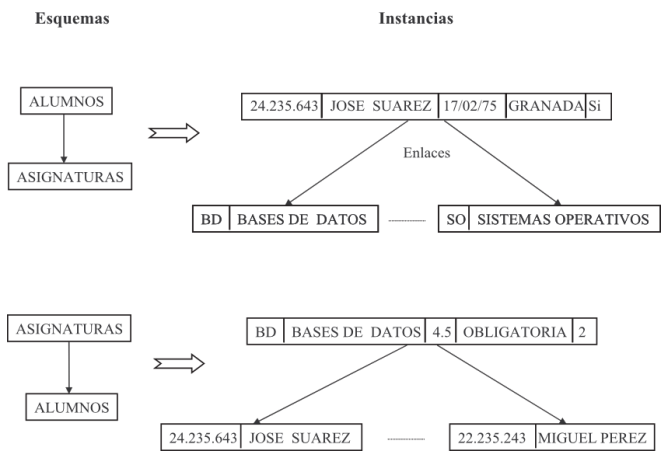
\includegraphics[scale=1,width=0.8\textwidth]{modelo_jerarquico.png}
\caption{Ejemplo de modelo jerárquico}
\end{figure}

Esta estructura plasma de forma muy directa las relaciones muchos a uno y las relaciones uno a uno. Sin embargo, en las relaciones muchos a muchos hay que duplicar toda la información sobre las entidades involucradas. \\

Como inconvenientes de este modelo encontramos que almacenar árboles en ficheros es comlejo, debido a los distintos tipos de registros y los punteros que hay que mantener. Además el DML es difícil de usar e implementar. Otro inconveniente es la dependencia existencial obligatoria de los registros de tipo secundario con respecto a los de tipo raíz, es decir, no se podrá insertar un registro de tipo secundario mientras no exista uno de tipo raíz con el que enlazarlo. Como ya hemos dicho antes en las relaciones muchos a muchos es necesaria la redundancia, lo que implica que la integridad de los datos es costosa de mantener. \\

\textbf{Modelo en red:} la estructura de datos son grafos cuya topología depende de las conexiones existentes entre las entidades:

\begin{itemize}
\item Nodos:registros.
\item Arcos: enlaces entre registros (punteros).
\item Relaciones entre conjuntos de entidades:
	
	\begin{itemize}
		\item Conectores: registros especiales (atributos propios de la relación). Cada ocurencia de un conector representa una asociación distintas.
	\end{itemize}
\end{itemize}

\begin{figure}[h]
\centering
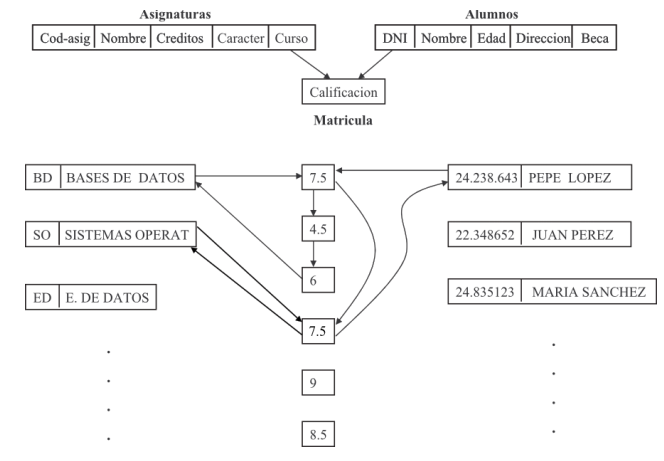
\includegraphics[scale=1,width=0.8\textwidth]{modelo_red.png}
\caption{Ejemplo de modelo en red}
\end{figure}


Por tanto la base de datos con un modelo en red es una colección de instancias de grafos. La estructura es muy genérica lo que permite plasmar todo tipo de relaciones e implementar directamente las relaciones muchos a muchos. \\

Como ventajas de este modelo tenemos que la estructura es algo más homogénea y que permite insertar nuevas entidades en un conjunto de forma independiente. Como problemas encontramos que la existencia de enlaces entre los registros hace que las operación del DDL y el DML sigan siendo complejas de implementar y utilizar. \\

\textbf{Comparativa:}
Haremos una comparativa entre el modelo relacional y los basados en grafos atendiendo a la representación y a la consulta:

\begin{itemize}
\item Con respecto a la representación: 
	\begin{itemize}
		\item En los modelos relacionales se requiere de un solo elemento para la representación (esencialidad), mientras que los basados en grafos requieren dos elementos para la representación.
		\item Los modelos relaciones tiene conexiones lógicas, mientras que los modelos basados en grafos tienen conexiones en el modelo físico subyacente.
		\item En el modelo relacional la representación de relaciones n:m es simétrica, mientras que en el basado en grafos la representación de estos es imposible en los modelos jerárquicos y difícil en los modelos de red.
		\item En el modelo relacional se tiene una identidad por valor, mientras que en los basados en grafos se tiene una identidad por posición.
	\end{itemize}
	
\item Con respecto a la consulta:
	\begin{itemize}
		\item En los modelos relacionales las consultas son simétricas en jerarquías, mientras que en los basados en grafos las consultas son no simétricas en jerarquías.
		\item En los modelos relacionales la obtención de la consulta es el resultado global (lenguaje declarativo), mientras que los basados en grafos disponen de un mecanismo de navegación por punteros (lenguaje procedimental)
	\end{itemize}
\end{itemize}

\textbf{Orientación a objetos:}
Los SGBD relacionales tiene las siguientes debilidades:
\begin{itemize}
\item Pobre representación de las entidades del mundo real.
\item Sobrecarga semántica de la estructura básica, la relación.
\item La estructura relacional es muy estrica. Todas las tuplas han de tener los mismo atributos, los valores  de un atributo pertenecen al mismo dominio y los atributos han de tener un valor atómico.
\item SQL permite un conjunto de operaciones limitado. No permite modelar el comportamiento de muchos objetos del mundo real.

\item Object-relational impedance mismatch: problemas conceptuale sy técnicos que se presentan a menudo al trabajar con sistemas gestores de bases de datos relacionales desde servidores de aplicaciones desarrollados en lenguajes orientados a objetos.
\end{itemize}

La filosofía del modelado orientado a objetos es abstraer un modelo de la realidad en forma de conjunto de objetos que interaccionan entre sí por medio de mensajes. Conceptos:

\begin{itemize}
\item Estado / comportamiento
\item Propiedades / métodos
\item Encapsulamiento 
\item Herencia
\item Polimorfismo
\end{itemize}

\begin{figure}[h]
\centering
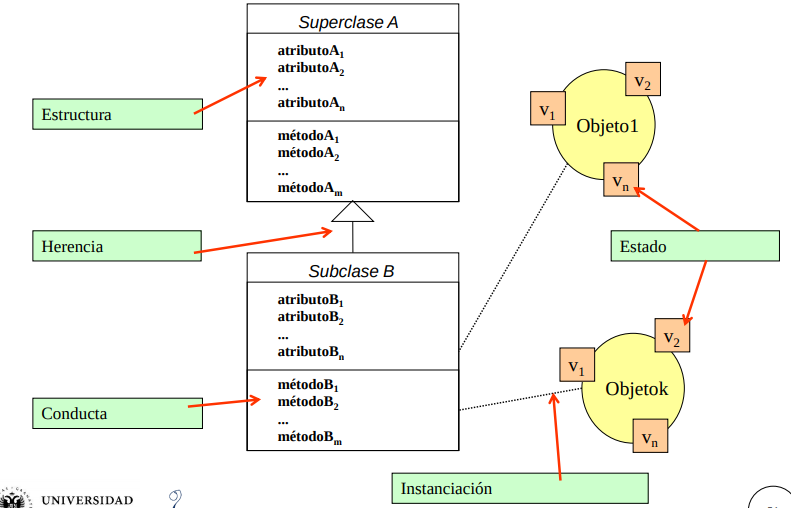
\includegraphics[scale=1,width=0.8\textwidth]{ejemplo_orientado_objetos.png}
\end{figure}

En el mundo de las bases de datos encontramos la siguiente jerarquía:

\begin{enumerate}
\item Orientación a objetos. Tiene una gran capacidad de modelado pero muestra dificultades de implementación del SGBD.

\item Objeto-relacional. Solidez de SGBD relacionales y una gran capacidad de modelado de la orientacióna a objetos.
\end{enumerate}

Normalmente las empresas usan uno de los siguientes modelos de BD:

\begin{itemize}
\item Bases de datos operacionales (Modelos relacional o de objetos o OLTP).
\item Bases de datos analíticas (Modelo multidimensional o OLAP).
\end{itemize}

\textbf{OLTP: On-line Transaction Processing:} las aplicaciones OLTP proporcionan soporte a operaciones diarias: estructuradas, repetitivas. Requieren datos detallados y el día. Las operaciones afectan fundamentalmente a pocos registros a los cuales se accede principalmente a través de la clave primaria. En este modelo es de vital importancia mantener la consistencia y la fiabilidad. El criterio esencial de rendimiento es optimizar la gestión de transacciones. \\

\textbf{OLAP: On-line analytical processing} las aplicaciones OLAP estan orientadas al soporte de decisiones y no son tan previsibles. Entre los datos más importantes de este tipo de bases de datos encontramos los datos consolidados, los resumidos y los de tipos histórico. Estos sistemas necesitan resolver consultas complejas, fundamentalmente consultas 'ad hoc', aunque también predefinidas, y puede involucrar a millones de registros. Este tipo de bases de datos necesita estructuras de datos diferentes. El procesamineto de consultas y el tiempo de respuesta son más importantes que el control de transacciones.

\begin{figure}[h]
\centering
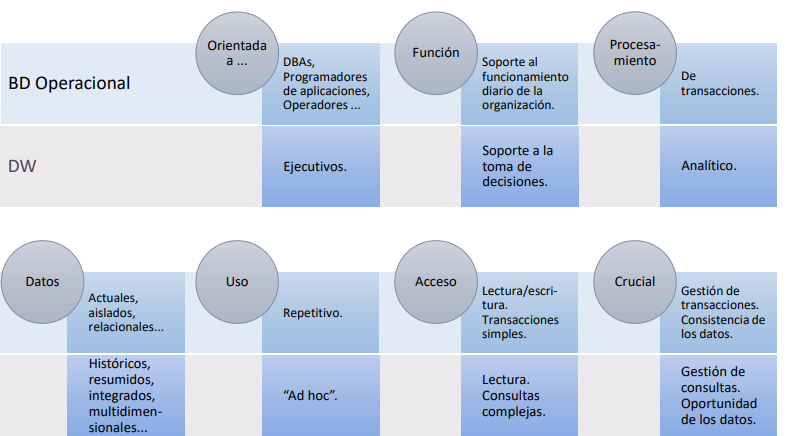
\includegraphics[scale=1,width=1\textwidth]{comparacion.png}
\caption{Comparación entre una BD relacional y una analítica}
\end{figure}

\textbf{Cubo de datos-Sistemas multidimensionales}:

El modelado dimensional es una técnica de modelado que permite organizar los datos como un conjunto de medidas que están descritas por aspectos comunes del negocio. Es de probada utilidad para agregar/desagregar datos y reordenarlos para el análisis. Este modelado está enfocado para trabajar sobre datos numéricos (valores, conteos, ratios, ...). Si se compara con otros modelos más propios de sistemas operacionales (modelado E/R, diagramas de clases, o modelos de datos lógicos como el relacional o el objeto-relacional), puede considerarse más fácil de entender y usar (es más sencillo) y visualmente más atractivo.

\begin{figure}[h]
\centering
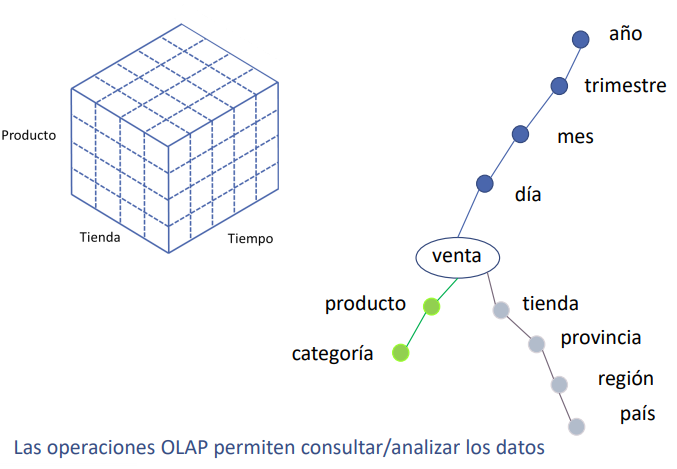
\includegraphics[scale=1,width=1\textwidth]{modelado_dimensional.png}
\end{figure}

\end{document}